\begin{figure}[htbp]
    \centering
    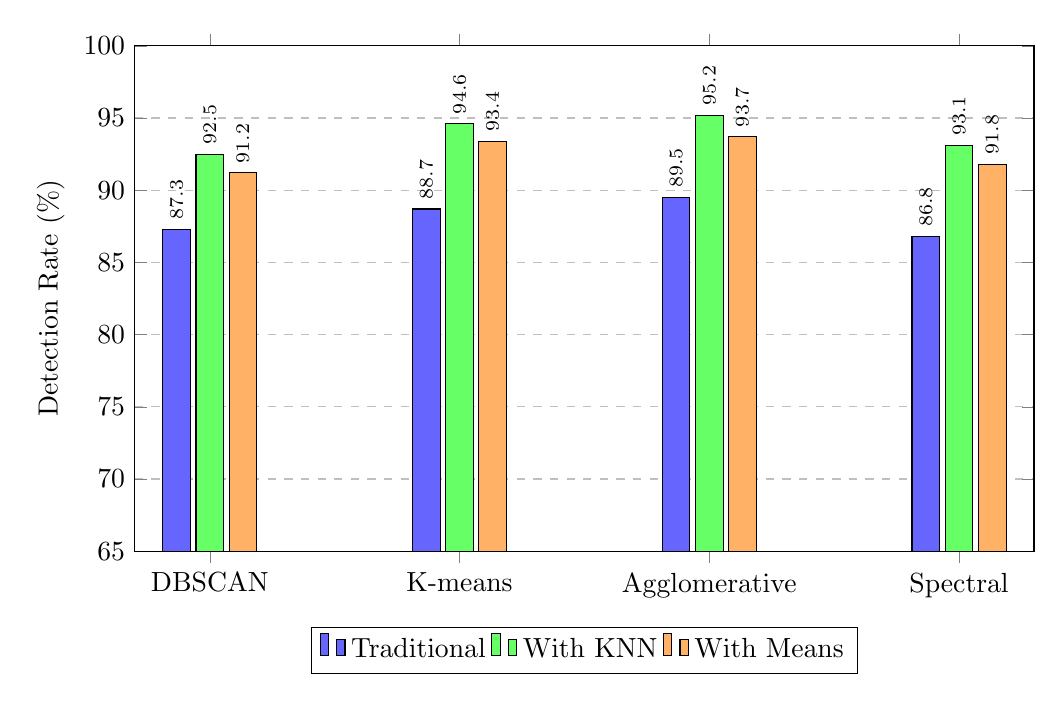
\begin{tikzpicture}
        \begin{axis}[
            width=13cm,
            height=8cm,
            ybar,
            bar width=10pt,
            ylabel={Detection Rate (\%)},
            symbolic x coords={DBSCAN, K-means, Agglomerative, Spectral},
            xtick=data,
            ymin=65, ymax=100,
            legend style={at={(0.5,-0.15)}, anchor=north, legend columns=3},
            ylabel near ticks,
            ymajorgrids=true,
            grid style=dashed,
            nodes near coords,
            every node near coord/.append style={font=\scriptsize, rotate=90, anchor=west},
            ]
            
            \addplot[fill=blue!60, draw=black] coordinates {
                (DBSCAN, 87.3)
                (K-means, 88.7)
                (Agglomerative, 89.5)
                (Spectral, 86.8)
            };
            \addlegendentry{Traditional}
            
            \addplot[fill=green!60, draw=black] coordinates {
                (DBSCAN, 92.5)
                (K-means, 94.6)
                (Agglomerative, 95.2)
                (Spectral, 93.1)
            };
            \addlegendentry{With KNN}
            
            \addplot[fill=orange!60, draw=black] coordinates {
                (DBSCAN, 91.2)
                (K-means, 93.4)
                (Agglomerative, 93.7)
                (Spectral, 91.8)
            };
            \addlegendentry{With Means}
            
        \end{axis}
    \end{tikzpicture}
    \caption{Detection rate comparison between traditional clustering algorithms and their enhanced versions in Scenario A (Far)}
    \label{fig:detection_comparison_A}
\end{figure}

\begin{figure}[htbp]
    \centering
    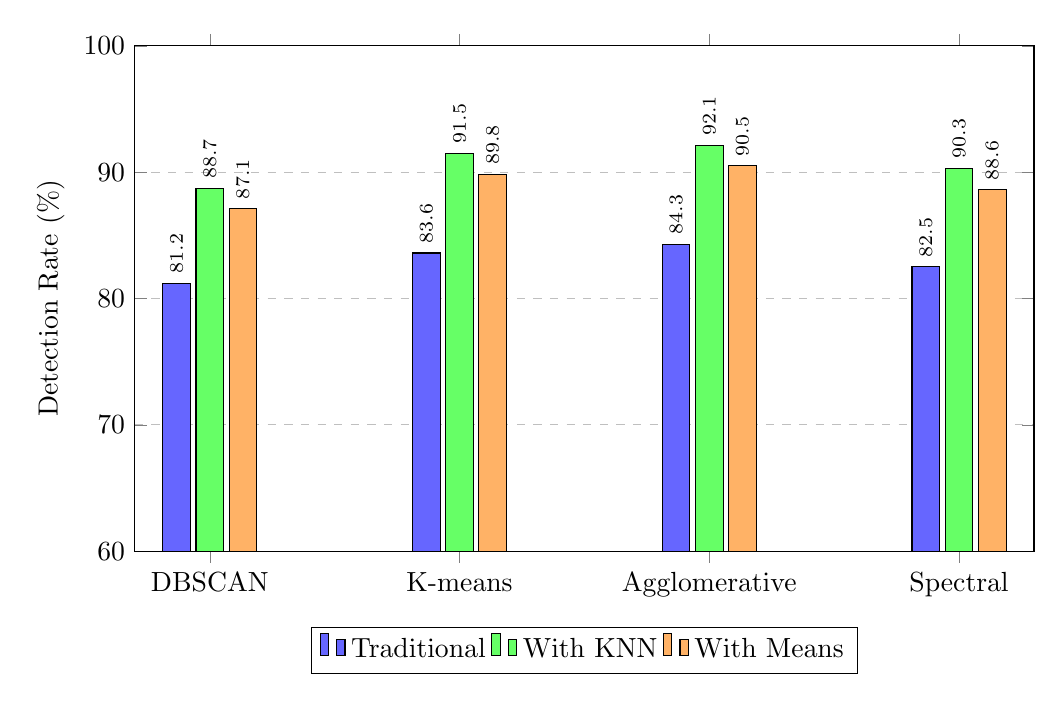
\begin{tikzpicture}
        \begin{axis}[
            width=13cm,
            height=8cm,
            ybar,
            bar width=10pt,
            ylabel={Detection Rate (\%)},
            symbolic x coords={DBSCAN, K-means, Agglomerative, Spectral},
            xtick=data,
            ymin=60, ymax=100,
            legend style={at={(0.5,-0.15)}, anchor=north, legend columns=3},
            ylabel near ticks,
            ymajorgrids=true,
            grid style=dashed,
            nodes near coords,
            every node near coord/.append style={font=\scriptsize, rotate=90, anchor=west},
            ]
            
            \addplot[fill=blue!60, draw=black] coordinates {
                (DBSCAN, 81.2)
                (K-means, 83.6)
                (Agglomerative, 84.3)
                (Spectral, 82.5)
            };
            \addlegendentry{Traditional}
            
            \addplot[fill=green!60, draw=black] coordinates {
                (DBSCAN, 88.7)
                (K-means, 91.5)
                (Agglomerative, 92.1)
                (Spectral, 90.3)
            };
            \addlegendentry{With KNN}
            
            \addplot[fill=orange!60, draw=black] coordinates {
                (DBSCAN, 87.1)
                (K-means, 89.8)
                (Agglomerative, 90.5)
                (Spectral, 88.6)
            };
            \addlegendentry{With Means}
            
        \end{axis}
    \end{tikzpicture}
    \caption{Detection rate comparison between traditional clustering algorithms and their enhanced versions in Scenario B (Medium)}
    \label{fig:detection_comparison_B}
\end{figure}

\begin{figure}[htbp]
    \centering
    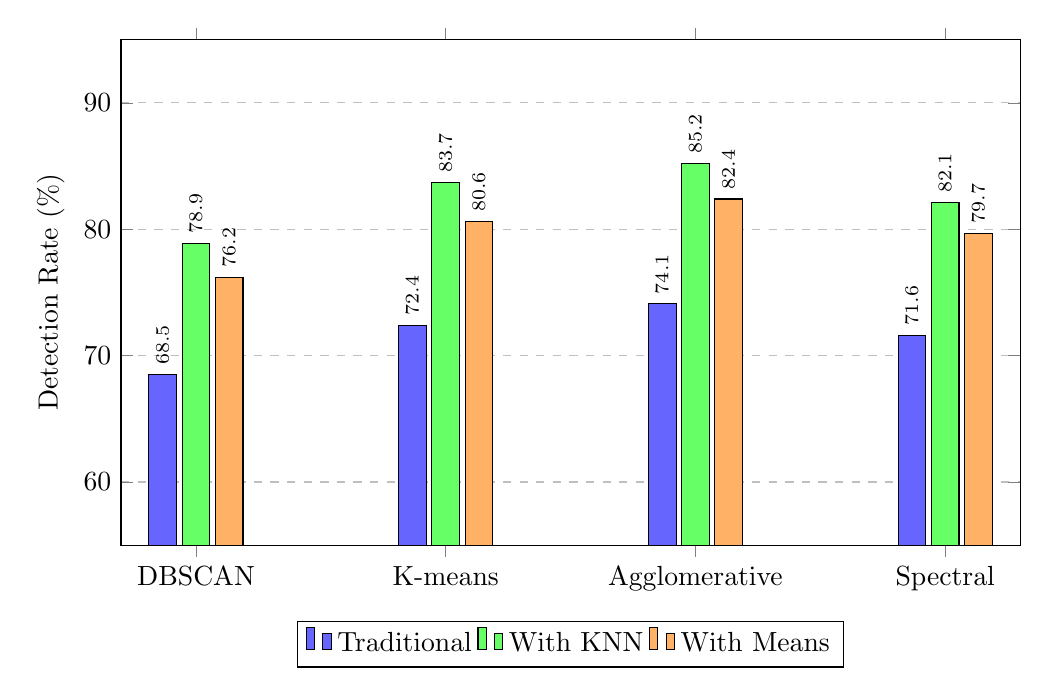
\begin{tikzpicture}
        \begin{axis}[
            width=13cm,
            height=8cm,
            ybar,
            bar width=10pt,
            ylabel={Detection Rate (\%)},
            symbolic x coords={DBSCAN, K-means, Agglomerative, Spectral},
            xtick=data,
            ymin=55, ymax=95,
            legend style={at={(0.5,-0.15)}, anchor=north, legend columns=3},
            ylabel near ticks,
            ymajorgrids=true,
            grid style=dashed,
            nodes near coords,
            every node near coord/.append style={font=\scriptsize, rotate=90, anchor=west},
            ]
            
            \addplot[fill=blue!60, draw=black] coordinates {
                (DBSCAN, 68.5)
                (K-means, 72.4)
                (Agglomerative, 74.1)
                (Spectral, 71.6)
            };
            \addlegendentry{Traditional}
            
            \addplot[fill=green!60, draw=black] coordinates {
                (DBSCAN, 78.9)
                (K-means, 83.7)
                (Agglomerative, 85.2)
                (Spectral, 82.1)
            };
            \addlegendentry{With KNN}
            
            \addplot[fill=orange!60, draw=black] coordinates {
                (DBSCAN, 76.2)
                (K-means, 80.6)
                (Agglomerative, 82.4)
                (Spectral, 79.7)
            };
            \addlegendentry{With Means}
            
        \end{axis}
    \end{tikzpicture}
    \caption{Detection rate comparison between traditional clustering algorithms and their enhanced versions in Scenario C (Close)}
    \label{fig:detection_comparison_C}
\end{figure}

\begin{figure}[htbp]
    \centering
    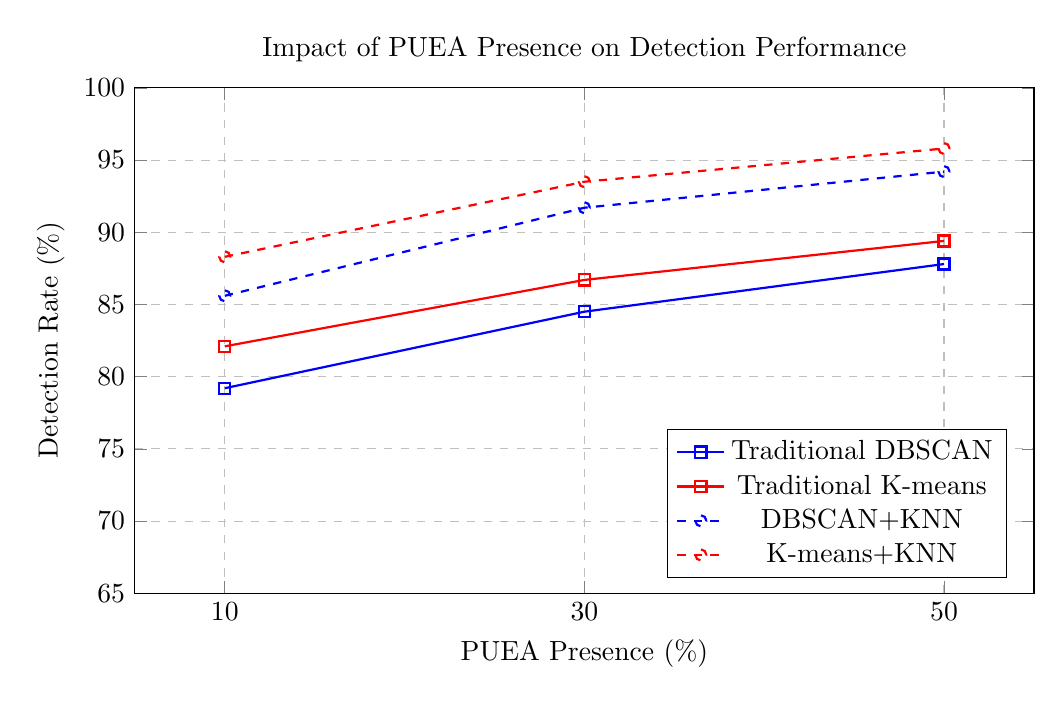
\begin{tikzpicture}
        \begin{axis}[
            width=13cm,
            height=8cm,
            xlabel={PUEA Presence (\%)},
            ylabel={Detection Rate (\%)},
            xmin=5, xmax=55,
            ymin=65, ymax=100,
            xtick={10,30,50},
            legend pos=south east,
            ymajorgrids=true,
            xmajorgrids=true,
            grid style=dashed,
            title={Impact of PUEA Presence on Detection Performance}
            ]
            
            % Traditional clustering lines
            \addplot[color=blue, mark=square, thick] coordinates {
                (10, 79.2)
                (30, 84.5)
                (50, 87.8)
            };
            \addlegendentry{Traditional DBSCAN}
            
            \addplot[color=red, mark=square, thick] coordinates {
                (10, 82.1)
                (30, 86.7)
                (50, 89.4)
            };
            \addlegendentry{Traditional K-means}
            
            % Enhanced clustering lines
            \addplot[color=blue, mark=o, thick, dashed] coordinates {
                (10, 85.6)
                (30, 91.7)
                (50, 94.2)
            };
            \addlegendentry{DBSCAN+KNN}
            
            \addplot[color=red, mark=o, thick, dashed] coordinates {
                (10, 88.3)
                (30, 93.5)
                (50, 95.8)
            };
            \addlegendentry{K-means+KNN}
            
        \end{axis}
    \end{tikzpicture}
    \caption{Detection rate as a function of PUEA presence percentage for traditional and enhanced clustering approaches}
    \label{fig:puea_presence_impact}
\end{figure}
